\documentclass[journal]{IEEEtran}

\usepackage{amsmath,amssymb,amsfonts}
\usepackage{algorithm}
\usepackage{algorithmic}
\usepackage{graphicx}
\usepackage{booktabs}
\usepackage{multirow}
\usepackage{array}
\usepackage{cite}
\usepackage{url}
\usepackage{xcolor}
\usepackage{balance}

\newcommand{\pchorch}{P3C-Orch}
\newcommand{\pclr}{P3C-LR Core}
\newcommand{\psr}{P3C-SR}
\newcommand{\etp}{ET-P3C}
\newcommand{\vect}[1]{\mathbf{#1}}
\newcommand{\norm}[1]{\widetilde{#1}}

\begin{document}

\title{Predictive 3C Orchestration for UAV-Swarm Low-Altitude IoT under Environmental Link Uncertainty}

% TODO: Replace author names, emails, ORCID, and affiliation before submission.
\author{First Author, Second Author, and Third Author% <-this % stops a space
\thanks{The authors are with the Department of Computer Science and Engineering, National Institute of Technology Meghalaya, India.}%
\thanks{Implementation availability details are given in the reproducibility note.}% TODO: Replace author metadata before submission.
}

\markboth{IEEE Internet of Things Journal, Draft Manuscript}{P3C-Orch for UAV-Swarm Low-Altitude IoT}

\maketitle

\begin{abstract}
UAV swarms can support low-altitude IoT services, but their links are affected by mobility, weather, and limited onboard resources. Existing works usually study caching, routing, deployment, or task collaboration separately. This paper presents \pchorch, a predictive computation, communication, and caching orchestration framework for heterogeneous UAV swarms under environmental link uncertainty. The framework uses an ANN-based link-risk predictor, cache-value-aware scheduling, and mobility-aware dwell control. The lightweight practical controller, \pclr, uses predicted link margin and outage risk together with cache value, energy cost, delay cost, load, and handover cost. We also study \psr, an internal stability-regularized variant, and \etp, an exploratory event-triggered ablation. On blind paper-lock seeds across seven regimes, \pclr\ ranks first against external baselines. Under combined stress, it improves the aggregate objective by 6.47\% over Reactive-3C, reduces average delay by 0.61\%, p95 delay by 2.14\%, handovers by 24.52\%, and outage by 9.14\%. These improvements over Reactive-3C are Holm-corrected significant for delay, p95 delay, handovers, and outage. The tradeoff is that \pclr\ uses 0.72\% more energy and has 1.05\% lower useful cache hit ratio than Reactive-3C. \psr\ achieves the best aggregate non-oracle objective, while \etp\ does not provide reliable additional gain. The results show that predictive 3C orchestration is useful, but it does not dominate every metric.
\end{abstract}

\begin{IEEEkeywords}
Low-altitude economy, UAV swarms, edge intelligence, 3C orchestration, caching, link-risk prediction, mobility-aware scheduling, Internet of Things.
\end{IEEEkeywords}

\section{Introduction}
Low-altitude economy (LAE) services use UAVs for sensing, delivery, monitoring, and emergency support. In such services, UAV swarms can act as flying edge nodes for IoT users and vehicles. They can relay data, serve local requests, cache popular content, and provide temporary communication coverage. UAV-assisted wireless networks are also a key topic in 5G and beyond systems because UAVs provide flexible deployment and good line-of-sight opportunities \cite{li2019uavcommunications}.

The main difficulty is that the service state changes quickly. Users move, content requests are bursty, UAV energy is limited, and air-to-ground links are affected by distance, altitude, speed mismatch, and weather. A scheduler that only maximizes the current rate may switch swarms too often. A scheduler that only minimizes energy may delay urgent demand. A cache-aware method may still fail when the cached content cannot be served over a risky link. Hence, computation, communication, and caching, called 3C resources in this paper, should be handled together.

Existing works address important parts of this problem. MUCCO jointly considers coded caching, user grouping, and UAV deployment for energy-efficient data delivery \cite{wei2025mucco}. A recent post-disaster UAV-swarm work uses collaborative beamforming, multi-path routing, and rate maximization for emergency communication \cite{zheng2025postdisaster}. Dynamic task collaboration studies asynchronous two-layer UAV-swarm control and stability for task-volume consensus \cite{zhou2026dynamic}. These works are useful references, but they do not directly address predictive cache-value-aware 3C scheduling under environmental link uncertainty and competing dynamic content demand.

This paper proposes \pchorch, a predictive 3C orchestration framework for heterogeneous UAV swarms. The framework uses an ANN to predict next-slot link margin and converts it into outage risk using weather-wise calibration. It then scores feasible swarm-cluster assignments using predicted link risk, useful cache value, delay, energy, load, fairness, and mobility-aware dwell cost. The main practical method is \pclr. We also study \psr, an internal stability-regularized variant, and \etp, an exploratory event-triggered ablation.

The contributions are as follows.
\begin{itemize}
    \item We build a predictive 3C orchestration model for heterogeneous UAV swarms serving moving low-altitude IoT demand under clear, rainy, and rain-hot weather.
    \item We integrate ANN-based link-risk prediction with weather-wise uncertainty calibration and use it inside the scheduling decision.
    \item We design \pclr, a cache-value-aware and mobility-aware controller that jointly considers link margin, outage, energy, delay, load, and handover cost.
    \item We report \psr\ as a stability-regularized internal variant and \etp\ as an exploratory ablation, without hiding negative or mixed results.
    \item We evaluate all methods on 80 blind paper-lock seeds across seven regimes and report confidence intervals and Holm-corrected statistical tests.
\end{itemize}

The rest of the paper is organized as follows. Section II reviews related work. Section III gives the system model. Section IV describes the ANN link-risk predictor. Sections V and VI present \pchorch\ and its algorithms. Section VII explains the experimental setup. Section VIII discusses the results. Section IX gives ablations and limitations. Section X concludes the paper.

\section{Related Work}
\subsection{UAV Caching and Data Delivery in LAE}
Caching can reduce repeated backhaul access and improve latency when content demand is skewed. The coded caching result in \cite{maddahali2014fundamental} provides a basic reference for cache-aided delivery. MUCCO is the closest LAE caching and deployment work for this paper. It jointly optimizes coded caching, user grouping, and UAV deployment, and it uses projected-distance-based grouping, semidefinite programming, and matching theory for energy-efficient data delivery \cite{wei2025mucco}. In contrast, \pchorch\ does not focus on coded caching design. It uses useful cache value as one part of a predictive service-assignment score that also includes link risk, dwell cost, delay, and energy.

\subsection{UAV Swarm Communication and Routing}
UAV-swarm communication has been studied for emergency and post-disaster networks. The post-disaster communication work in \cite{zheng2025postdisaster} builds a collaborative self-organizing network using collaborative beamforming, Ford-Fulkerson style routing, and diffusion-model-enabled particle swarm optimization. Its main goal is transmission-rate maximization. This motivates the RateMax baseline in our experiments. Our setting is different because users generate content requests over time and the scheduler must consider cache state, mobility-aware handover, and predicted link risk.

\subsection{UAV Swarm Task Collaboration and Stability}
Task collaboration among large UAV swarms is related to orchestration, but it has a different control objective. The work in \cite{zhou2026dynamic} proposes asynchronous two-layer task collaboration with energy constraints and Lyapunov-based analysis. It focuses on task-volume consensus and hierarchical collaboration. This paper does not claim a new consensus theorem. Instead, \pchorch\ schedules service assignments for communication, caching, and computation. We include \psr\ as a stability-regularized internal variant, but the final claim is based on measured paper-lock results.

\subsection{Link-Risk Prediction and Environmental Uncertainty}
Air-to-ground links depend on altitude, elevation angle, path loss, and line-of-sight probability. We use the standard low-altitude platform path-loss model in \cite{alhourani2014lap} as a basis for simulation. UAV energy and movement cost are also important, and UAV communication energy models such as \cite{zeng2019rotary} motivate including energy in the scheduler. Our project notes and user presentation reported clear, rainy, and rain-hot link-margin degradation, wider residuals in harsh weather, and link instability due to speed mismatch. Hence, \pchorch\ uses a link-margin predictor and weather-wise risk calibration rather than relying only on current observed margin.

\subsection{Summary of Gap}
Table~\ref{tab:related_work} summarizes the difference. Different from these works, \pchorch\ uses predicted link risk, useful cache value, dwell cost, delay, energy, and outage together for service assignment.

\begin{table*}[!t]
\centering
\caption{Comparison with closely related UAV-swarm and LAE works.}
\label{tab:related_work}
\tiny
\begin{tabular}{p{0.105\textwidth}p{0.105\textwidth}p{0.065\textwidth}p{0.115\textwidth}p{0.065\textwidth}p{0.105\textwidth}p{0.065\textwidth}p{0.155\textwidth}}
\toprule
Work & Main focus & Caching & Routing/communication & Prediction & Mobility/handover & 3C orchestration & Main limitation \\
\midrule
MUCCO~\cite{wei2025mucco} & Energy-efficient data delivery & Yes & Coverage and grouping & No & Mobility-aware deployment & Partial & No ANN link-risk prediction or dwell-aware multi-swarm predictive 3C scheduling \\
Post-disaster UAV swarm~\cite{zheng2025postdisaster} & Transmission-rate maximization & No & Collaborative beamforming and routing & No & Placement optimization & Partial & No cache-value-aware dynamic content scheduling \\
Dynamic task collaboration~\cite{zhou2026dynamic} & Task collaboration and consensus & No & Control network & No & Two-layer asynchronous control & No & Focuses on task-volume collaboration, not service-level 3C orchestration \\
P3C-Orch & Predictive service orchestration & Useful cache value & Link-risk-aware assignment & ANN link-risk & Dwell guard & Yes & Simulation-based; real UAV traces still needed \\
\bottomrule
\end{tabular}
\end{table*}


\section{System Model}
We consider a time-slotted UAV-swarm service system. Time slots are indexed by $t=1,2,\ldots,T$. A high-altitude platform or edge controller observes the state of heterogeneous UAV swarms, moving users, content requests, cache states, and weather. It then assigns UAV swarms to active demand clusters.

Let $\mathcal{S}=\{1,\ldots,S\}$ denote the set of UAV swarms. Each swarm $s\in\mathcal{S}$ has a position $\vect{p}_{s,t}$, bandwidth $W_s$, transmit power $P_s$, residual energy $E_{s,t}$, cache $\mathcal{C}_{s,t}$, service capacity, current load $L_{s,t}$, and previous assignments. The altitude is limited to $[h_{\min},h_{\max}]$. Users and vehicles move according to a Gauss--Markov mobility model, which is commonly used to represent correlated movement in mobile ad hoc simulations \cite{camp2002mobility}.

At slot $t$, active requesting users are grouped into demand clusters $\mathcal{K}_t$. Cluster $k\in\mathcal{K}_t$ has centroid $\vect{u}_{k,t}$, demand arrival $A_{k,t}$, deadline $\tau_{k,t}$, priority, requested files, and backlog $Q_{k,t}$. The binary variable $x_{s,k,t}\in\{0,1\}$ is one if swarm $s$ serves cluster $k$ at slot $t$. Each cluster is assigned to at most one swarm:
\begin{equation}
\sum_{s\in\mathcal{S}} x_{s,k,t} \leq 1, \quad \forall k\in\mathcal{K}_t.
\label{eq:assignment_one}
\end{equation}

The backlog evolves as
\begin{equation}
Q_{k,t+1}=\left[Q_{k,t}+A_{k,t}-\mu_{k,t}\right]^+,
\label{eq:queue_update}
\end{equation}
where $\mu_{k,t}=\sum_s x_{s,k,t}\mu_{s,k,t}$ is the served traffic and $[y]^+=\max(y,0)$. Traffic that remains after the deadline is counted as dropped.

The air-to-ground channel uses distance-based path loss, line-of-sight probability, weather attenuation, speed mismatch penalty, and random shadowing. Let $m_{s,k,t}$ be the observed link margin between swarm $s$ and cluster $k$. The service estimate is
\begin{equation}
\mu_{s,k,t}=R_{s,k,t}\left(1-\hat{p}^{\mathrm{out}}_{s,k,t}\right),
\label{eq:service_rate}
\end{equation}
where $R_{s,k,t}$ is the link capacity and $\hat{p}^{\mathrm{out}}_{s,k,t}$ is the predicted outage probability.

The cache value for a swarm-cluster pair is
\begin{align}
V^{\mathrm{cache}}_{s,k,t}={}&\left(1-\hat{p}^{\mathrm{out}}_{s,k,t}\right)
\Big(a_1H^{\mathrm{local}}_{s,k,t}+a_2H^{\mathrm{nbr}}_{s,k,t} \nonumber\\
&-a_3S_{s,k,t}-a_4N_{s,k,t}\Big),
\label{eq:cache_value}
\end{align}
where $H^{\mathrm{local}}$ is the valid local service hit ratio, $H^{\mathrm{nbr}}$ is the neighbor-cache reuse ratio, $S$ is a stale-cache penalty, and $N$ is a neighbor-fetch penalty. This form makes cache useful only when it can reduce delay or energy under the predicted link condition.

The switch cost is
\begin{equation}
C^{\mathrm{sw}}_{s,k,t}=\mathbb{1}\{s\neq s^{\mathrm{prev}}_{k,t}\}\left(c_0+c_1d_{s,k,t}+c_2\right),
\label{eq:switch_cost}
\end{equation}
where $s^{\mathrm{prev}}_{k,t}$ is the previous serving swarm of the persistent cluster and $d_{s,k,t}$ is the distance. No handover is counted for a newly born cluster. Energy and delay are represented as additive costs:
\begin{align}
C^{\mathrm{en}}_{s,k,t} &= C^{\mathrm{tx}}_{s,k,t}+C^{\mathrm{move}}_{s,k,t}+C^{\mathrm{fetch}}_{s,k,t},\label{eq:energy_cost}\\
D_{s,k,t} &= D^{\mathrm{deadline}}_{k,t}+D^{\mathrm{queue}}_{s,t}+D^{\mathrm{miss}}_{s,k,t}+\hat{p}^{\mathrm{out}}_{s,k,t}.\label{eq:delay_cost}
\end{align}
Table~\ref{tab:notation} lists the main symbols.

\begin{table}[!t]
\centering
\caption{Main notation used in the system model.}
\label{tab:notation}
\scriptsize
\begin{tabular}{ll}
\toprule
Symbol & Meaning \\
\midrule
$\mathcal{S}$ & Set of UAV swarms \\
$s$ & Index of a UAV swarm \\
$\mathcal{K}_t$ & Active demand clusters at slot $t$ \\
$k$ & Index of a demand cluster \\
$x_{s,k,t}$ & Binary assignment variable \\
$\mathcal{C}_{s,t}$ & Cache state of swarm $s$ \\
$Q_{k,t}$ & Backlog of demand cluster $k$ \\
$A_{k,t}$ & New arrival demand \\
$\mu_{s,k,t}$ & Expected service by swarm $s$ for cluster $k$ \\
$\hat{m}_{s,k,t+1}$ & Predicted next-slot link margin \\
$\hat{p}^{\mathrm{out}}_{s,k,t}$ & Predicted outage probability \\
$V^{\mathrm{cache}}_{s,k,t}$ & Useful cache value \\
$C^{\mathrm{en}}_{s,k,t}$ & Energy cost \\
$D_{s,k,t}$ & Delay cost \\
$C^{\mathrm{sw}}_{s,k,t}$ & Switch/handover cost \\
$B_{s,k,t}$ & P3C-LR Core scheduling score \\
\bottomrule
\end{tabular}
\end{table}


\section{ANN-Based Link-Risk Prediction}
The controller predicts the next-slot link margin before scheduling. For every feasible swarm-cluster pair, the feature vector $\vect{z}_{s,k,t}$ includes swarm and cluster identifiers, distance, elevation angle, relative speed, weather state, frequency, bandwidth, transmit power, previous link margin, previous outage flag, cache-hit flag, residual energy, current load, and normalized time. The ANN is an MLP with three hidden layers of 64 ReLU neurons. The output is the predicted next-slot link margin:
\begin{equation}
\hat{m}_{s,k,t+1}=f_{\theta}(\vect{z}_{s,k,t}).
\label{eq:ann_margin}
\end{equation}

The margin prediction is converted into outage risk using weather-wise residual calibration:
\begin{equation}
\hat{p}^{\mathrm{out}}_{s,k,t}=\sigma\left(\frac{m_{\mathrm{th}}-\hat{m}_{s,k,t+1}}{\sigma_w}\right),
\label{eq:outage_risk}
\end{equation}
where $m_{\mathrm{th}}$ is the outage margin threshold, $\sigma_w$ is the calibrated residual scale for weather state $w$, and $\sigma(\cdot)$ is the sigmoid function. This risk value is used in both service estimation and scheduling.

\begin{algorithm}[!t]
\caption{ANN-Based Link-Risk Prediction}
\label{alg:link_prediction}
\begin{algorithmic}[1]
\REQUIRE Feature vector $\vect{z}_{s,k,t}$, trained ANN $f_\theta$, weather state $w$, threshold $m_{\mathrm{th}}$, calibration scale $\sigma_w$
\ENSURE Predicted margin $\hat{m}_{s,k,t+1}$ and outage risk $\hat{p}^{\mathrm{out}}_{s,k,t}$
\STATE Collect distance, elevation angle, relative speed, weather, bandwidth, transmit power, previous margin, previous outage, cache flag, energy, load, and time features.
\STATE Normalize features using the predictor preprocessing rule.
\STATE Compute $\hat{m}_{s,k,t+1}=f_\theta(\vect{z}_{s,k,t})$.
\STATE Select weather-wise residual scale $\sigma_w$.
\STATE Compute $\hat{p}^{\mathrm{out}}_{s,k,t}=\sigma((m_{\mathrm{th}}-\hat{m}_{s,k,t+1})/\sigma_w)$.
\RETURN $\hat{m}_{s,k,t+1}$, $\hat{p}^{\mathrm{out}}_{s,k,t}$.
\end{algorithmic}
\end{algorithm}


The final paper-lock predictor results are shown in Tables~\ref{tab:predictor_metrics} and~\ref{tab:predictor_weather}. The overall RMSE is 4.592 dB and the Pearson correlation is 0.810. Weather-wise errors are not identical. The rain-hot state has the largest RMSE in the paper-lock predictor table, which matches the motivation that harsh weather causes wider residuals.

\begin{table}[!t]
\centering
\caption{Overall ANN link-margin predictor metrics on the paper-lock predictor evaluation set.}
\label{tab:predictor_metrics}
\scriptsize
\begin{tabular}{lccccc}
\toprule
MSE & RMSE & MAE & $R^2$ & Pearson $R$ & Time/sample (ms) \\
\midrule
21.090 & 4.592 & 3.865 & 0.554 & 0.810 & 0.0042 \\
\bottomrule
\end{tabular}
\end{table}

\begin{table}[!t]
\centering
\caption{Weather-wise link predictor error and calibrated residual scale.}
\label{tab:predictor_weather}
\scriptsize
\begin{tabular}{lcccccc}
\toprule
Weather & MSE & RMSE & MAE & $R^2$ & Samples & $\sigma_w$ (dB) \\
\midrule
clear & 20.194 & 4.494 & 3.910 & 0.510 & 1332 & 4.711 \\
rain\_hot & 24.200 & 4.919 & 3.900 & 0.512 & 346 & 4.310 \\
rainy & 21.232 & 4.608 & 3.777 & 0.522 & 822 & 4.108 \\
\bottomrule
\end{tabular}
\end{table}


Fig.~\ref{fig:predictor_scatter} shows the predicted and true link margins, and Fig.~\ref{fig:predictor_residual} shows residuals by weather. These figures are used as predictor diagnostics and not as proof that the link model is complete.

\begin{figure}[!t]
\centering
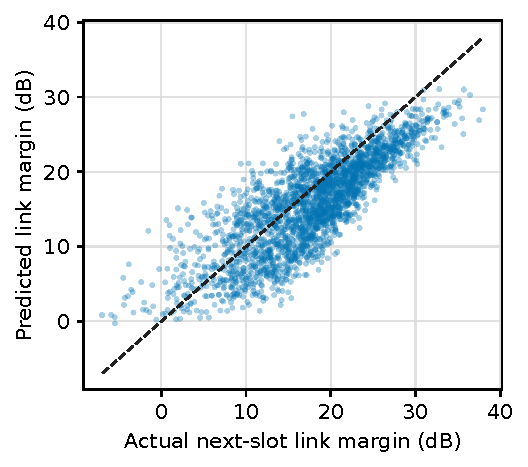
\includegraphics[width=\columnwidth]{figs/predictor_scatter_paperlock.pdf}
\caption{ANN link-margin prediction scatter on the paper-lock predictor evaluation set. The plot compares predicted and actual margins. The spread shows that prediction is useful but not exact.}
\label{fig:predictor_scatter}
\end{figure}

\begin{figure}[!t]
\centering
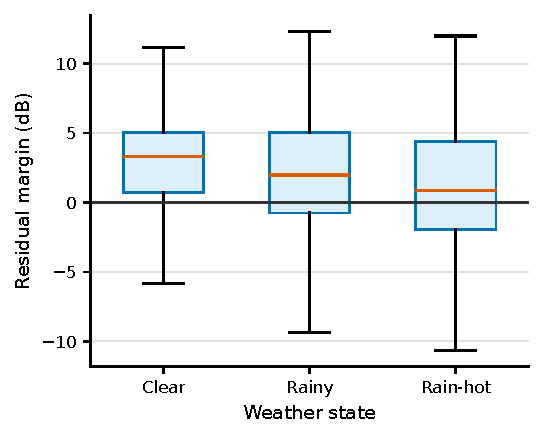
\includegraphics[width=\columnwidth]{figs/predictor_residual_by_weather_paperlock.pdf}
\caption{Prediction residuals by weather state. The rain-hot condition has wider error spread than easier weather states, so outage risk calibration is needed.}
\label{fig:predictor_residual}
\end{figure}

\section{P3C-Orch Framework}
Fig.~\ref{fig:system_model} shows the \pchorch\ system model. The controller receives mobility, cache, load, energy, and link states from the UAV swarms and demand clusters. It predicts next-slot link margin, estimates outage risk, computes cache value, applies dwell control, and assigns each active demand cluster to a feasible swarm.

\begin{figure}[!t]
\centering
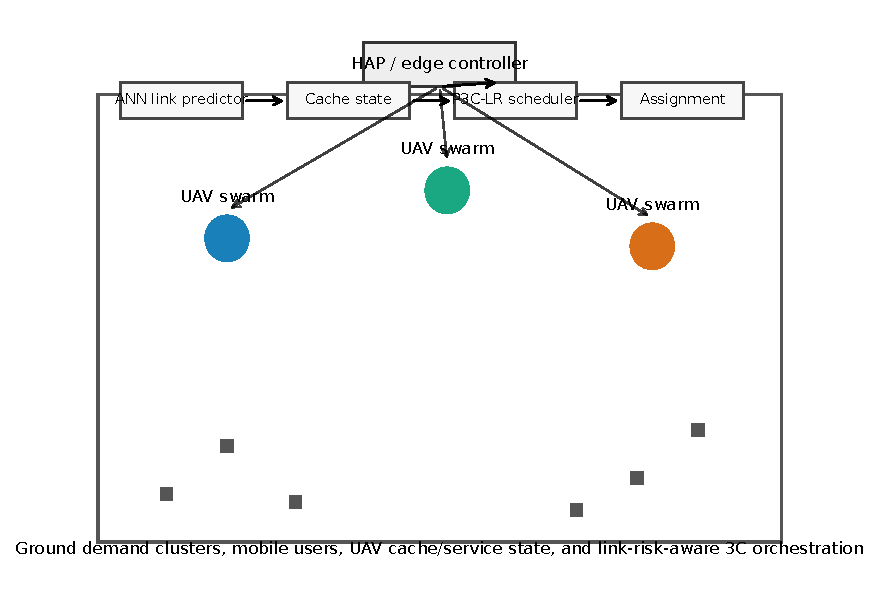
\includegraphics[width=\columnwidth]{figs/system_model_p3clr.pdf}
\caption{System model of \pchorch. Ground users generate content requests, UAV swarms provide service and cache reuse, and the edge controller uses link prediction, cache state, and scheduling state for assignment.}
\label{fig:system_model}
\end{figure}

\begin{figure}[!t]
\centering
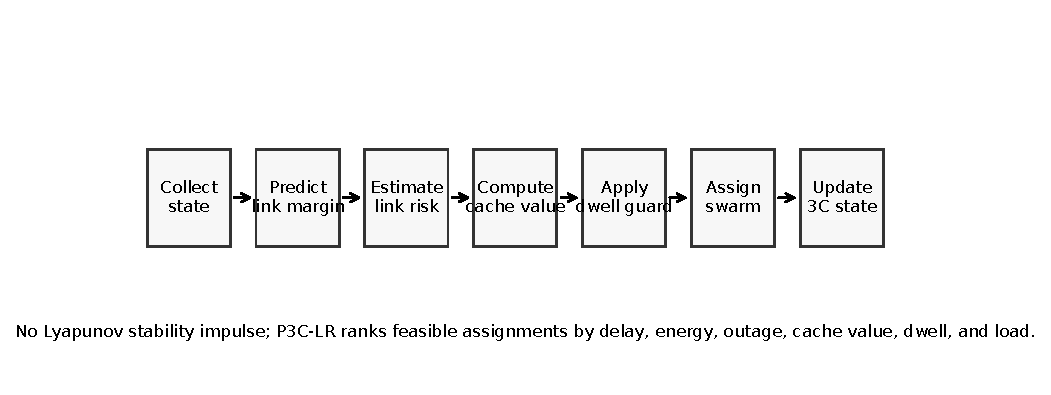
\includegraphics[width=\columnwidth]{figs/algorithm_flow_p3clr.pdf}
\caption{Algorithm flow of \pchorch. The controller collects state, predicts link risk, computes cache value and dwell cost, assigns swarms, and updates queue, cache, energy, and handover states.}
\label{fig:algorithm_flow}
\end{figure}

For \pclr, every feasible swarm-cluster pair receives a normalized score:
\begin{align}
B_{s,k,t}={}&w_m\norm{m}_{s,k,t}+w_c\norm{V}^{\mathrm{cache}}_{s,k,t}+w_f\norm{F}_{s,t}+w_r\norm{R}^{\mathrm{dwell}}_{s,k,t}\nonumber\\
&-w_d\norm{D}_{s,k,t}-w_e\norm{C}^{\mathrm{en}}_{s,k,t}-w_o\norm{p}^{\mathrm{out}}_{s,k,t}\nonumber\\
&-w_h\norm{C}^{\mathrm{sw}}_{s,k,t}-w_l\norm{L}_{s,t}.
\label{eq:p3clr_score}
\end{align}
Here, $\norm{m}$ is the normalized risk-adjusted link margin, $\norm{V}^{\mathrm{cache}}$ is normalized useful cache value, $\norm{F}$ is a fairness term, $\norm{R}^{\mathrm{dwell}}$ rewards staying with the previous feasible swarm, $\norm{D}$ is delay cost, $\norm{C}^{\mathrm{en}}$ is energy cost, $\norm{p}^{\mathrm{out}}$ is outage risk, $\norm{C}^{\mathrm{sw}}$ is switching cost, and $\norm{L}$ is swarm load. The normalization is done per slot over feasible pairs so that no single raw scale dominates the score.

The scheduling problem is
\begin{align}
\max_{x_{s,k,t}} &\quad \sum_{k\in\mathcal{K}_t}\sum_{s\in\mathcal{S}} x_{s,k,t}B_{s,k,t} \label{eq:assignment_problem}\\
\mathrm{s.t.} &\quad \sum_s x_{s,k,t}\leq 1,\quad \forall k,\nonumber\\
&\quad \sum_k x_{s,k,t}\mu_{s,k,t}\leq \bar{\mu}_{s,t},\quad \forall s,\nonumber\\
&\quad x_{s,k,t}\in\{0,1\}.\nonumber
\end{align}
The implementation uses greedy assignment ordered by deadline-aware urgency and backlog for scalability. A dwell guard keeps the previous swarm if it remains feasible and if the new score gain is too small to justify a handover. This guard is important because KMeans-like cluster movement can otherwise create unnecessary handovers.

The paper objective is used only for ranking the final results, not for tuning on paper-lock seeds:
\begin{align}
J={}&0.18\norm{D}_{\mathrm{avg}}+0.16\norm{D}_{95}+0.16\norm{E}+0.14\norm{H}\nonumber\\
&+0.12\norm{p}^{\mathrm{out}}+0.10\norm{P}_{\mathrm{drop}}+0.08\norm{I}_{\mathrm{load}}\nonumber\\
&-0.08\norm{H}^{\mathrm{cache}}-0.08\norm{T}_{\mathrm{put}}-0.04\norm{F}_{\mathrm{Jain}}.
\label{eq:paper_objective}
\end{align}
A lower value of $J$ is better. Individual metrics are always reported with the objective.

\section{P3C-SR and Internal Variants}
\pclr\ is the lightweight practical controller. We also study \psr, which adds a stability regularizer to the same predictive 3C score. The regularizer is
\begin{equation}
G_{s,k,t}=U_{k,t}\mu_{s,k,t}-\lambda L_{s,t}\mu_{s,k,t},
\label{eq:stability_gain}
\end{equation}
where $U_{k,t}=Q_{k,t}/\max(\tau_{k,t}-t+1,1)$ is the deadline-aware urgency and $L_{s,t}$ is the swarm load. The \psr\ score is
\begin{equation}
B^{\mathrm{SR}}_{s,k,t}=B_{s,k,t}+w_q\norm{G}_{s,k,t}.
\label{eq:p3csr_score}
\end{equation}
The term is a regularizer and not the only design objective. It can help when backlog and deadline risk are high, but it can also affect energy, cache use, and throughput. Therefore, we report \psr\ as an internal variant rather than replacing the practical core.

\etp\ was also tested as an exploratory event-triggered ablation. It activates a bounded stability impulse only under high-risk states. In the paper-lock results, \etp\ is close to \pclr\ and \psr, but it does not give a clear statistically reliable gain. Hence, \etp\ is not used as the main method.

\begin{algorithm}[!t]
\caption{\pclr\ Scheduling}
\label{alg:p3clr}
\begin{algorithmic}[1]
\REQUIRE Swarm states, demand clusters, cache states, trained link predictor, dwell parameters
\ENSURE Assignment $x_{s,k,t}$ and updated queue, cache, energy, and handover states
\STATE Form active demand clusters and persistent cluster identifiers.
\FOR{each feasible pair $(s,k)$}
    \STATE Predict link margin and outage risk using Algorithm~\ref{alg:link_prediction}.
    \STATE Estimate expected service $\mu_{s,k,t}$.
    \STATE Compute useful local and neighbor cache value.
    \STATE Compute delay, energy, load, fairness, dwell, and switch costs.
    \STATE Normalize all score terms over feasible pairs in the current slot.
    \STATE Compute $B_{s,k,t}$ using \eqref{eq:p3clr_score}.
\ENDFOR
\STATE Sort clusters by deadline-aware urgency and backlog.
\FOR{each cluster in sorted order}
    \STATE Select the feasible swarm with the largest score.
    \STATE Apply dwell guard; keep the previous swarm when it is feasible and the score gain is small.
    \STATE Commit assignment if capacity and energy constraints are satisfied.
\ENDFOR
\STATE Serve traffic and update $Q_{k,t+1}$ using \eqref{eq:queue_update}.
\STATE Update cache, energy, load, delay, outage, drop, and handover counters.
\end{algorithmic}
\end{algorithm}

\begin{algorithm}[!t]
\caption{\psr\ Stability-Regularized Scheduling}
\label{alg:p3csr}
\begin{algorithmic}[1]
\REQUIRE Same inputs as Algorithm~\ref{alg:p3clr}, stability weight $w_q$, load regularization $\lambda$
\ENSURE Stability-regularized assignment and updated states
\STATE Build all feasible pair terms as in Algorithm~\ref{alg:p3clr}.
\FOR{each feasible pair $(s,k)$}
    \STATE Compute urgency $U_{k,t}=Q_{k,t}/\max(\tau_{k,t}-t+1,1)$.
    \STATE Compute $G_{s,k,t}=U_{k,t}\mu_{s,k,t}-\lambda L_{s,t}\mu_{s,k,t}$.
    \STATE Normalize $G_{s,k,t}$ over feasible pairs.
    \STATE Compute $B^{\mathrm{SR}}_{s,k,t}=B_{s,k,t}+w_q\norm{G}_{s,k,t}$.
\ENDFOR
\STATE Assign clusters using the same greedy order and dwell guard.
\STATE Update queue, cache, energy, outage, delay, and handover states.
\end{algorithmic}
\end{algorithm}


\section{Experimental Setup}
The experiment uses the final paper-lock outputs only. The simulator is time-slotted and uses a $1000\,\mathrm{m}\times1000\,\mathrm{m}$ area with heterogeneous UAV swarms, moving users, dynamic content requests, finite caches, and Markov weather. The altitude range is $100$--$200$ m. Users move with Gauss--Markov mobility and request files from a Zipf-distributed library. Demand clusters are formed from active requesting users.

The evaluated regimes are: R1 normal load, R2 near saturation, R3 overload, R4 severe burst, R5 harsh weather, R6 high mobility, and R7 combined stress. The main paper discussion focuses on harsh weather, high mobility, and combined stress, but all regimes are reported.

The compared methods are Random, Nearest, RateMax, MUCCO-like, Reactive-3C, \pclr, \psr, \etp, OracleLink Upper Bound, and OracleSelector Upper Bound. OracleLink uses true next-slot link margin. OracleSelector uses hindsight selection. Both are upper bounds and are excluded from practical ranking.

The paper-lock blind seeds are $4001$--$4080$, giving 80 paired runs per regime and method. Earlier seeds from Pilot-0, v2, and v3 are treated only as development evidence. No tuning was run on the paper-lock seeds. The seed audit passed all checks, including seed disjointness, frozen configuration before the run, no tuning, identical seeds/regimes for all methods, and exclusion of Oracle methods from practical ranking. The implementation will be made available at: \url{https://github.com/Devchandrasen/p3c-orch}. % GitHub link set for the project repository.

The primary metrics are average delay, p95 delay, total energy consumption, handovers per 100 active cluster-slots, useful cache hit ratio, outage probability, throughput, and drop rate. Secondary metrics include backlog, SLA violations, load imbalance, fairness, computation overhead, and predictor error. Results are reported as mean $\pm$ 95\% confidence interval over the blind seeds when available.

\section{Results and Discussion}
\subsection{Link-Risk Prediction Performance}
The ANN predictor gives an overall RMSE of 4.592 dB, MAE of 3.865 dB, and Pearson correlation of 0.810. Weather-wise RMSE is 4.494 dB for clear, 4.608 dB for rainy, and 4.919 dB for rain-hot. This supports the use of weather-wise calibration, but it also shows that harsh-weather prediction remains imperfect.

\subsection{Main Result Against External Baselines}
Table~\ref{tab:main_results} gives the combined-stress paper-lock results. \pclr\ has objective 0.684, while Reactive-3C has 0.731. This is a 6.47\% objective improvement over Reactive-3C. \pclr\ reduces average delay by 0.61\%, p95 delay by 2.14\%, handovers by 24.52\%, and outage by 9.14\%. The corrected p-values are 0.00653 for average delay, $7.60\times10^{-7}$ for p95 delay, $2.53\times10^{-7}$ for handovers, and 0.0285 for outage. These are treated as statistically reliable.

\pclr\ does not dominate all metrics. Compared with Reactive-3C, it increases energy consumption by 0.72\%, reduces useful cache hit ratio by 1.05\%, and increases drop rate by 0.53\%. The energy difference is Holm-corrected significant, but it is a worsening for \pclr. The useful cache and drop-rate differences are not corrected significant in the Reactive-3C comparison.

\begin{table*}[!t]
\centering
\caption{Combined-stress paper-lock results on blind seeds 4001--4080. Energy is in kJ. Cache, outage, and drop are in percent. Oracle methods are upper bounds and excluded from practical ranking.}
\label{tab:main_results}
\tiny
\begin{tabular}{lccccccccc}
\toprule
Method & Avg Delay & p95 Delay & Energy & Handovers/100 & Useful Cache & Outage & Drop & Throughput & Objective \\
\midrule
Random & 6.32 $\pm$ 0.05 & \textbf{7.70 $\pm$ 0.08} & 20.19 $\pm$ 0.20 & 58.15 $\pm$ 0.48 & 0.00 $\pm$ 0.00 & 1.31 $\pm$ 0.10 & 41.55 $\pm$ 1.91 & 598.3 $\pm$ 4.7 & 2.995 $\pm$ 0.025 \\
Nearest & 6.52 $\pm$ 0.04 & 7.89 $\pm$ 0.08 & 19.50 $\pm$ 0.27 & \textbf{1.33 $\pm$ 0.16} & 0.00 $\pm$ 0.00 & \textbf{0.23 $\pm$ 0.02} & 42.17 $\pm$ 1.82 & 591.6 $\pm$ 8.8 & 0.732 $\pm$ 0.012 \\
RateMax & 6.40 $\pm$ 0.04 & 7.72 $\pm$ 0.07 & 20.19 $\pm$ 0.20 & 34.40 $\pm$ 0.60 & 0.00 $\pm$ 0.00 & 0.82 $\pm$ 0.06 & 43.08 $\pm$ 1.94 & 583.5 $\pm$ 4.7 & 2.085 $\pm$ 0.024 \\
MUCCO-like & 6.28 $\pm$ 0.07 & 8.06 $\pm$ 0.09 & \textbf{16.57 $\pm$ 0.15} & 17.49 $\pm$ 0.54 & 26.63 $\pm$ 0.62 & 0.79 $\pm$ 0.07 & \textbf{37.29 $\pm$ 1.93} & \textbf{653.4 $\pm$ 5.7} & 1.228 $\pm$ 0.024 \\
Reactive-3C & 6.26 $\pm$ 0.07 & 8.02 $\pm$ 0.10 & 16.69 $\pm$ 0.14 & 3.86 $\pm$ 0.22 & \textbf{27.71 $\pm$ 0.60} & 0.96 $\pm$ 0.07 & 37.98 $\pm$ 1.91 & 643.8 $\pm$ 5.7 & 0.731 $\pm$ 0.018 \\
P3C-LR Core & \textbf{6.22 $\pm$ 0.07} & 7.85 $\pm$ 0.10 & 16.81 $\pm$ 0.16 & 2.92 $\pm$ 0.22 & 27.42 $\pm$ 0.68 & 0.88 $\pm$ 0.06 & 38.18 $\pm$ 1.84 & 643.4 $\pm$ 6.5 & 0.684 $\pm$ 0.016 \\
P3C-SR & 6.24 $\pm$ 0.07 & 7.87 $\pm$ 0.10 & 16.89 $\pm$ 0.15 & 2.77 $\pm$ 0.19 & 27.45 $\pm$ 0.63 & 0.81 $\pm$ 0.05 & 37.82 $\pm$ 1.90 & 647.3 $\pm$ 6.2 & \textbf{0.671 $\pm$ 0.016} \\
ET-P3C & 6.22 $\pm$ 0.07 & 7.84 $\pm$ 0.10 & 16.82 $\pm$ 0.15 & 2.76 $\pm$ 0.19 & 27.44 $\pm$ 0.67 & 0.88 $\pm$ 0.06 & 38.13 $\pm$ 1.83 & 643.4 $\pm$ 6.3 & 0.680 $\pm$ 0.017 \\
\textit{OracleLink Upper Bound} & \textit{6.21 $\pm$ 0.07} & \textit{7.85 $\pm$ 0.10} & \textit{16.82 $\pm$ 0.15} & \textit{3.95 $\pm$ 0.25} & \textit{27.58 $\pm$ 0.62} & \textit{0.87 $\pm$ 0.06} & \textit{38.11 $\pm$ 1.89} & \textit{643.9 $\pm$ 6.1} & \textit{0.720 $\pm$ 0.019} \\
\textit{OracleSelector Upper Bound} & \textit{6.26 $\pm$ 0.06} & \textit{7.85 $\pm$ 0.09} & \textit{17.96 $\pm$ 0.17} & \textit{11.20 $\pm$ 0.74} & \textit{19.99 $\pm$ 0.83} & \textit{0.73 $\pm$ 0.05} & \textit{39.33 $\pm$ 2.00} & \textit{658.4 $\pm$ 4.1} & \textit{1.020 $\pm$ 0.032} \\
\bottomrule
\end{tabular}
\end{table*}

\begin{table*}[!t]
\centering
\caption{Percentage change of P3C-LR Core against external baselines under combined stress. Positive values favour P3C-LR Core; negative values show worsening.}
\label{tab:external_baseline}
\scriptsize
\begin{tabular}{lccccccccc}
\toprule
Baseline & Avg Delay & p95 Delay & Energy & Handovers & Useful Cache & Outage & Drop & Throughput & Objective \\
\midrule
Reactive-3C & +0.61\% & +2.14\% & -0.72\% & +24.52\% & -1.05\% & +9.14\% & -0.53\% & -0.06\% & +6.47\% \\
MUCCO-like & +1.01\% & +2.56\% & -1.44\% & +83.33\% & +2.96\% & -11.40\% & -2.38\% & -1.54\% & +44.32\% \\
RateMax & +2.89\% & -1.67\% & +16.77\% & +91.52\% & n/a & -6.22\% & +11.37\% & +10.27\% & +67.20\% \\
\bottomrule
\end{tabular}
\end{table*}


\subsection{Comparison with MUCCO-like and RateMax}
Compared with MUCCO-like, \pclr\ improves the objective by 44.32\%, average delay by 1.01\%, p95 delay by 2.56\%, handovers by 83.33\%, and useful cache hit ratio by 2.96\%. It uses 1.44\% more energy, has 11.40\% higher outage, and has 2.38\% higher drop rate. This shows that MUCCO-like remains strong on energy and drop rate, but it has much higher handover cost in this dynamic setting.

Compared with RateMax, \pclr\ improves the objective by 67.20\%, average delay by 2.89\%, energy by 16.77\%, handovers by 91.52\%, drop rate by 11.37\%, and throughput by 10.27\%. However, RateMax has 1.67\% better p95 delay and 6.22\% lower outage in the combined-stress table. Thus, rate maximization alone is not enough for the aggregate energy-latency-handover objective, but it can still help some tail or outage metrics.

\subsection{Internal Variant Analysis}
Table~\ref{tab:internal_variant} compares \pclr, \psr, and \etp. \psr\ achieves the best aggregate non-oracle objective, 0.671, and is therefore the strongest overall non-oracle method by the paper objective. \pclr\ is the lightweight core and ranks first against external baselines. \etp\ is close to both methods but does not provide reliable additional gain. The manuscript therefore presents \pchorch\ as a framework containing the practical core and the stability-regularized internal variant.

\begin{table*}[!t]
\centering
\caption{Internal P3C-Orch variant comparison under combined stress. Energy is in kJ and ratio metrics are in percent.}
\label{tab:internal_variant}
\scriptsize
\begin{tabular}{lccccccccc}
\toprule
Variant & Avg Delay & p95 Delay & Energy & Handovers & Useful Cache & Outage & Drop & Throughput & Objective \\
\midrule
P3C-LR Core & 6.22 & 7.85 & 16.81 & 2.92 & 27.42 & 0.88 & 38.18 & 643.4 & 0.684 \\
P3C-SR & 6.24 & 7.87 & 16.89 & 2.77 & 27.45 & 0.81 & 37.82 & 647.3 & 0.671 \\
ET-P3C & 6.22 & 7.84 & 16.82 & 2.76 & 27.44 & 0.88 & 38.13 & 643.4 & 0.680 \\
\bottomrule
\end{tabular}
\end{table*}


\subsection{Regime-Wise Behaviour}
Fig.~\ref{fig:delay_cdf} shows the delay CDF under the paper-lock evaluation. Figs.~\ref{fig:energy_regime} and~\ref{fig:handover_regime} show energy and handover behaviour by regime. \pclr\ is useful when link risk and handover decisions matter, but the gains vary by regime. The regime-wise table is generated in \texttt{tables/regime\_results.tex} and retained for detailed checking.

\begin{figure}[!t]
\centering
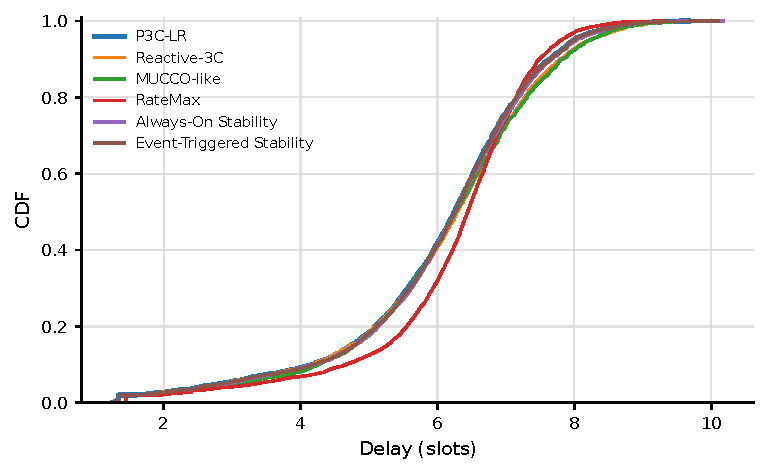
\includegraphics[width=\columnwidth]{figs/delay_cdf_paperlock.pdf}
\caption{Delay CDF for the main methods. The figure compares external baselines and internal variants under the final paper-lock evaluation.}
\label{fig:delay_cdf}
\end{figure}

\begin{figure}[!t]
\centering
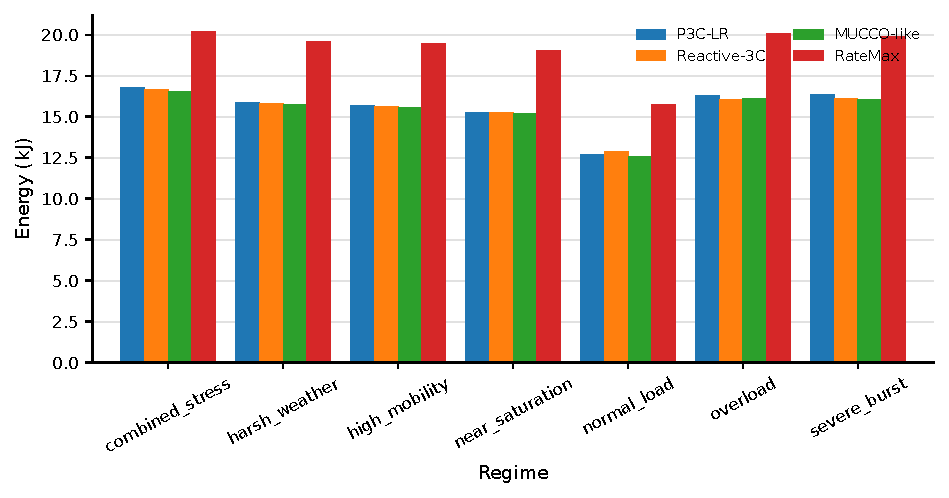
\includegraphics[width=\columnwidth]{figs/energy_by_regime_paperlock.pdf}
\caption{Energy consumption by regime. \pclr\ improves the aggregate objective against external baselines but has a small energy cost compared with Reactive-3C under combined stress.}
\label{fig:energy_regime}
\end{figure}

\begin{figure}[!t]
\centering
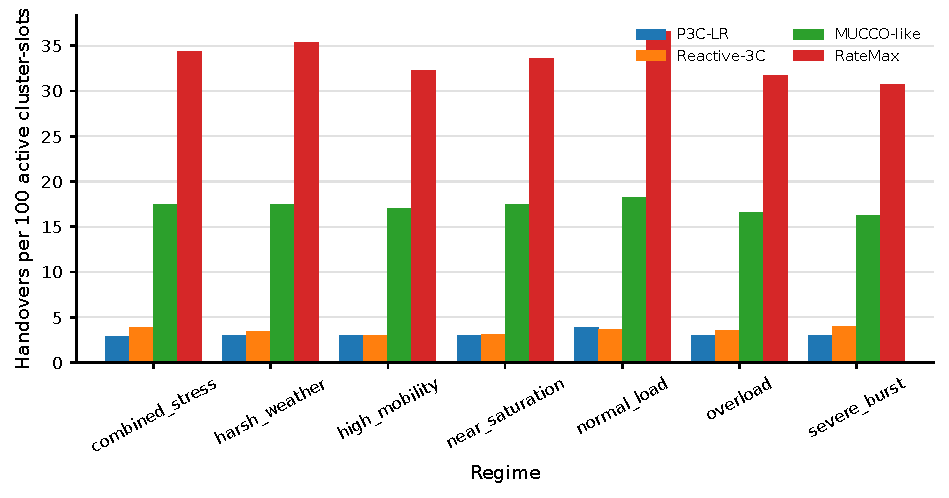
\includegraphics[width=\columnwidth]{figs/handover_by_regime_paperlock.pdf}
\caption{Handovers per 100 active cluster-slots by regime. Mobility-aware dwell control reduces unnecessary switching compared with rate-centric and caching-centric baselines.}
\label{fig:handover_regime}
\end{figure}

\subsection{Cache, Weather, and Oracle Gap}
Fig.~\ref{fig:cache_breakdown} shows cache-hit behaviour. Cache value helps when a hit reduces delay or energy, but \pclr\ can lose useful cache hit ratio against Reactive-3C because the scheduler also gives weight to outage and dwell. Fig.~\ref{fig:outage_weather} shows outage by weather. Fig.~\ref{fig:oracle_gap} shows the gap to upper bounds. Oracle methods are not practical baselines and are used only to show remaining headroom.

\begin{figure}[!t]
\centering
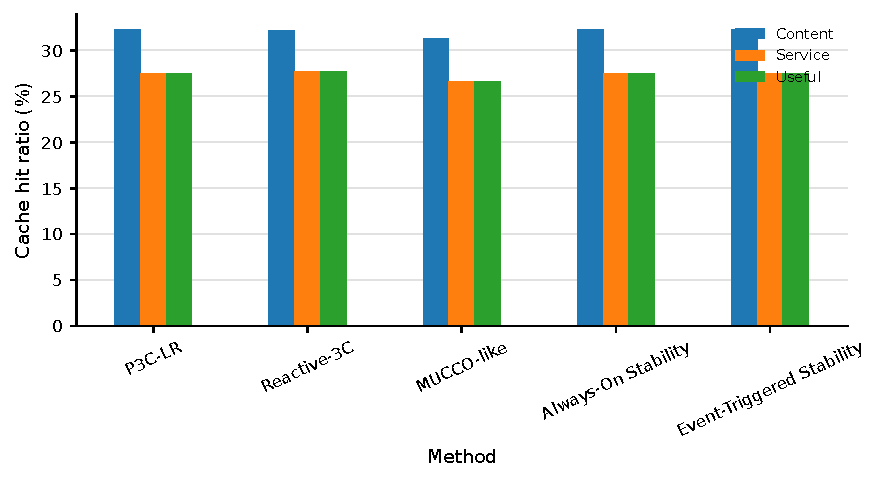
\includegraphics[width=\columnwidth]{figs/cache_hit_breakdown_paperlock.pdf}
\caption{Cache hit breakdown for the main methods. The figure separates cache effects instead of treating every cached file as useful.}
\label{fig:cache_breakdown}
\end{figure}

\begin{figure}[!t]
\centering
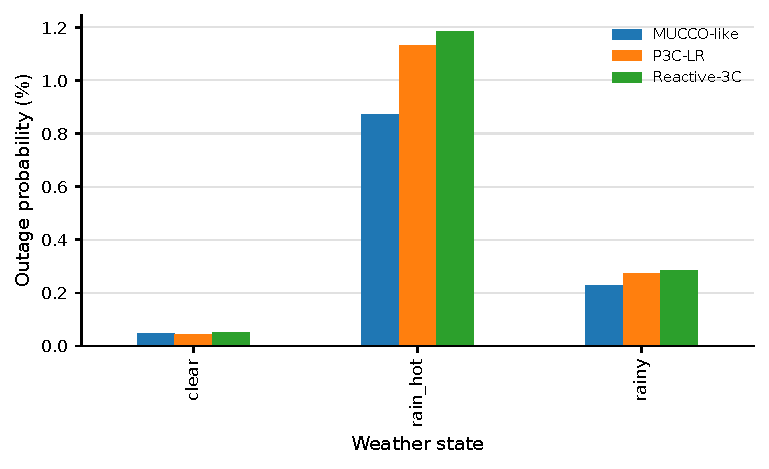
\includegraphics[width=\columnwidth]{figs/outage_by_weather_paperlock.pdf}
\caption{Outage behaviour by weather. Harsh weather increases link risk, which motivates prediction and calibration.}
\label{fig:outage_weather}
\end{figure}

\begin{figure}[!t]
\centering
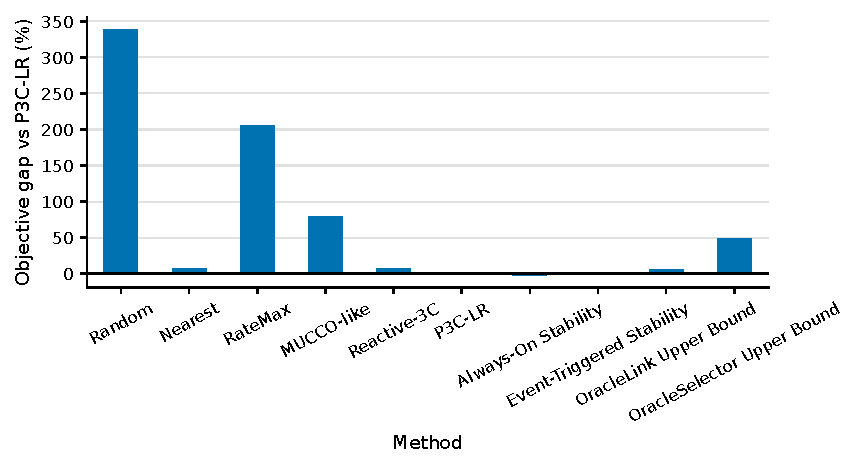
\includegraphics[width=\columnwidth]{figs/oracle_gap_paperlock.pdf}
\caption{Oracle gap under the paper-lock objective. OracleLink and OracleSelector are upper bounds and are excluded from practical ranking.}
\label{fig:oracle_gap}
\end{figure}

\subsection{Statistical Significance}
Only Holm-corrected significant results are treated as statistically reliable. Table~\ref{tab:significance} reports the corrected p-values. The main supported improvements over Reactive-3C are average delay, p95 delay, handovers, and outage. Energy is also corrected significant, but it is worse for \pclr. Hence, the main claim is a latency-handover-outage tradeoff, not universal dominance.

\begin{table*}[!t]
\centering
\caption{Holm-corrected Wilcoxon tests comparing P3C-LR Core with each baseline under combined stress. The Yes column only marks corrected $p<0.05$ and does not imply that the direction favours P3C-LR Core.}
\label{tab:significance}
\tiny
\begin{tabular}{llccc}
\toprule
Baseline & Metric & Corrected $p$ & Effect $d_z$ & $p<0.05$ \\
\midrule
Reactive-3C & Avg delay & 0.00653 & -0.417 & Yes \\
Reactive-3C & p95 delay & 7.6e-07 & -0.719 & Yes \\
Reactive-3C & Energy & 0.0211 & +0.404 & Yes \\
Reactive-3C & Handovers & 2.53e-07 & -0.780 & Yes \\
Reactive-3C & Useful cache & 1 & -0.161 & No \\
Reactive-3C & Outage & 0.0285 & -0.382 & Yes \\
Reactive-3C & Drop rate & 1 & +0.227 & No \\
Reactive-3C & Throughput & 1 & -0.043 & No \\
MUCCO-like & Avg delay & 5.69e-06 & -0.701 & Yes \\
MUCCO-like & p95 delay & 3.54e-07 & -0.761 & Yes \\
MUCCO-like & Energy & 5.97e-07 & +0.778 & Yes \\
MUCCO-like & Handovers & 3.14e-13 & -5.492 & Yes \\
MUCCO-like & Useful cache & 0.00178 & +0.426 & Yes \\
MUCCO-like & Outage & 0.0258 & +0.304 & Yes \\
MUCCO-like & Drop rate & 3.12e-09 & +0.918 & Yes \\
MUCCO-like & Throughput & 4.03e-09 & -0.945 & Yes \\
RateMax & Avg delay & 8.04e-09 & -0.891 & Yes \\
RateMax & p95 delay & 0.0276 & +0.412 & Yes \\
RateMax & Energy & 3.14e-13 & -7.536 & Yes \\
RateMax & Handovers & 3.14e-13 & -10.877 & Yes \\
RateMax & Useful cache & 3.14e-13 & +8.806 & Yes \\
RateMax & Outage & 0.202 & +0.210 & No \\
RateMax & Drop rate & 3.14e-13 & -3.375 & Yes \\
RateMax & Throughput & 3.14e-13 & +2.738 & Yes \\
P3C-SR & Avg delay & 0.623 & -0.246 & No \\
P3C-SR & p95 delay & 1 & -0.125 & No \\
P3C-SR & Energy & 0.0558 & -0.368 & No \\
P3C-SR & Handovers & 1 & +0.145 & No \\
P3C-SR & Useful cache & 1 & -0.020 & No \\
P3C-SR & Outage & 0.024 & +0.344 & Yes \\
P3C-SR & Drop rate & 0.0313 & +0.368 & Yes \\
P3C-SR & Throughput & 0.00644 & -0.477 & Yes \\
ET-P3C & Avg delay & 1 & -0.095 & No \\
ET-P3C & p95 delay & 1 & +0.034 & No \\
ET-P3C & Energy & 1 & -0.065 & No \\
ET-P3C & Handovers & 1 & +0.179 & No \\
ET-P3C & Useful cache & 1 & -0.017 & No \\
ET-P3C & Outage & 1 & -0.013 & No \\
ET-P3C & Drop rate & 1 & +0.077 & No \\
ET-P3C & Throughput & 1 & -0.001 & No \\
\bottomrule
\end{tabular}
\end{table*}


\subsection{Main Observations}
\begin{itemize}
    \item Link-risk prediction is useful when weather and mobility change the service quality.
    \item Mobility-aware dwell control reduces unnecessary handovers.
    \item Cache value helps when cached content reduces delay or energy, but cache hit ratio can drop when link-risk and dwell terms dominate.
    \item \psr\ gives the best aggregate non-oracle objective, but it does not remove all tradeoffs.
    \item \etp\ did not give reliable additional gain in this implementation.
\end{itemize}

\section{Ablation Study and Limitations}
\subsection{Ablation Study}
Table~\ref{tab:ablation} and Fig.~\ref{fig:ablation} show the ablation results. Removing ANN prediction increases delay and p95 delay. Removing cache value removes useful cache hit ratio and increases energy. Removing mobility-aware dwell gives lower average delay in this specific table, but it increases handovers sharply to 24.02 per 100 active cluster-slots. Removing neighbor cache almost halves the useful cache hit ratio. These results support the use of prediction, useful cache value, and dwell control as practical components of \pchorch.

\begin{table*}[!t]
\centering
\caption{Ablation results under combined stress. Energy is in kJ and ratio metrics are in percent.}
\label{tab:ablation}
\scriptsize
\begin{tabular}{lcccccccc}
\toprule
Variant & Avg Delay & p95 Delay & Energy & Handovers & Useful Cache & Outage & Drop & Throughput \\
\midrule
P3C-LR Core & 6.26 & 7.94 & 16.87 & 2.99 & 28.16 & 0.88 & 38.18 & 647.3 \\
No ANN prediction & 6.33 & 8.12 & 16.78 & 3.65 & 27.51 & 0.91 & 37.87 & 649.3 \\
No cache value & 6.46 & 8.12 & 20.21 & 3.35 & 0.00 & 0.79 & 38.39 & 645.4 \\
No mobility-aware dwell & 6.18 & 8.02 & 16.65 & 24.02 & 27.69 & 0.67 & 38.17 & 649.3 \\
No link-risk calibration & 6.28 & 8.14 & 16.64 & 2.95 & 28.47 & 0.96 & 38.03 & 644.3 \\
No neighbor cache & 6.29 & 7.94 & 17.28 & 3.09 & 14.21 & 0.90 & 38.52 & 643.3 \\
P3C-SR & 6.29 & 7.97 & 16.94 & 2.71 & 28.21 & 0.81 & 37.88 & 651.6 \\
ET-P3C & 6.26 & 7.91 & 16.93 & 2.60 & 27.80 & 0.91 & 38.14 & 647.1 \\
\bottomrule
\end{tabular}
\end{table*}


\begin{figure}[!t]
\centering
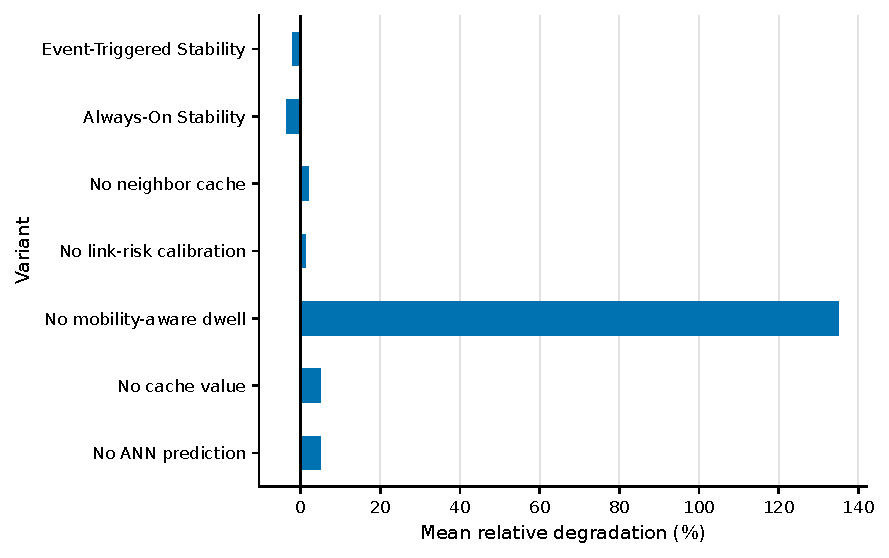
\includegraphics[width=\columnwidth]{figs/ablation_paperlock.pdf}
\caption{Ablation results for \pchorch. The figure shows the effect of removing prediction, cache value, dwell control, risk calibration, and neighbor cache reuse.}
\label{fig:ablation}
\end{figure}

\subsection{Stability Branch Analysis}
Fig.~\ref{fig:stability_branch} summarizes the stability branch. \psr\ is the stability-regularized internal variant and has the best aggregate non-oracle objective. However, earlier stability-focused branches did not give a clean, statistically reliable stability claim across all metrics. \etp\ is therefore reported as an exploratory ablation. This is why the paper is positioned as predictive 3C orchestration under link uncertainty, not as a pure stability-aware paper.

\begin{figure}[!t]
\centering
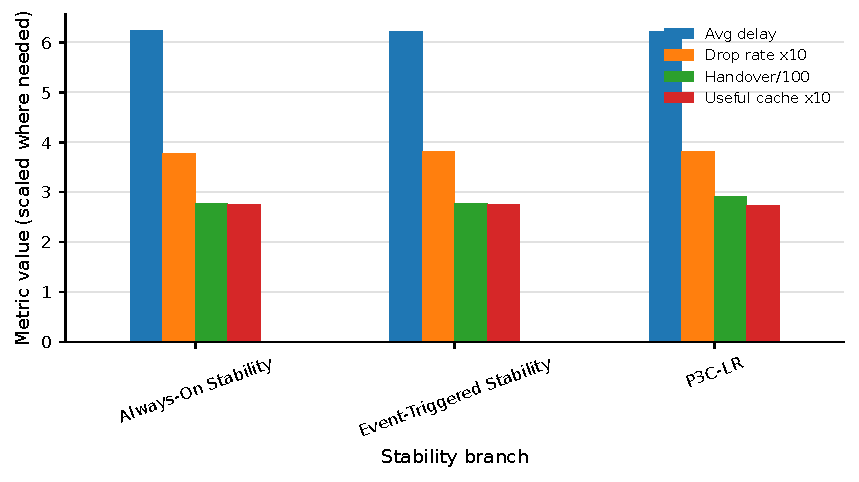
\includegraphics[width=\columnwidth]{figs/stability_negative_result_paperlock.pdf}
\caption{Stability branch analysis. \psr\ gives the best aggregate non-oracle objective, while \etp\ remains an exploratory ablation without a clear reliable gain over the simpler core.}
\label{fig:stability_branch}
\end{figure}

\subsection{Limitations}
This work has several limitations. First, the validation is simulation-based. Real UAV tests are needed before deployment. Second, the ANN predictor is trained on generated link data rather than real UAV field traces. Third, the weather model uses simplified clear, rainy, and rain-hot states. Fourth, security and privacy are not considered. Fifth, inter-UAV interference and detailed physical-layer beamforming are simplified. Sixth, \pclr\ does not improve every metric; it has a small energy cost and slightly lower useful cache hit ratio and drop-rate performance in some comparisons. Seventh, \etp\ did not provide reliable gain. Finally, real deployment will need hardware tests, controller delay measurement, and communication-delay validation.

These limitations do not remove the main result, but they define the next steps. Future work should use real link traces, online learning, interference-aware modelling, energy harvesting, and secure orchestration.

\section{Conclusion}
This paper presented \pchorch, a predictive 3C orchestration framework for UAV-swarm low-altitude IoT under environmental link uncertainty. The framework combines ANN-based link-risk prediction, cache-value-aware scheduling, mobility-aware dwell control, and optional stability regularization. The practical core, \pclr, ranks first against external baselines on the paper-lock objective. Against Reactive-3C, it reduces delay, p95 delay, handovers, and outage, with corrected statistical support for these metrics. It also has tradeoffs: energy consumption is slightly higher and useful cache hit ratio and drop rate are slightly worse. \psr\ gives the best aggregate non-oracle objective, while \etp\ is an exploratory ablation without reliable extra gain. Future work will focus on real trace validation, online adaptation, interference-aware link models, energy harvesting, and security-aware service orchestration.


\balance
\bibliographystyle{IEEEtran}
\bibliography{refs/references}

\end{document}
